\section{Sensor model}
\subsection{Radar sensor}
In this work a simple radar model is used. The radar is assumed to be able to detect things within a cone with a given spread and maximum range. The radar will give out the distance to the nearest object that overlaps the cone. Where inside the cone the object is, is unknown, only the distance to the object and the fact that the object is inside the cone is known. Figure \ref{fig:SensorData} shows the data gathered from 5 radar sensors. Black indicates that there is an obstacle that reflected the radar beam at that distance. White is safe areas where no obstacle has been detected. Gray is areas with no information. The radar beams are here made thinner to be able to distinguish them in the figure. In the rest of this paper, the radars will be made thicker such that the gap between them is removed. Figure \ref{fig:SuperimposedSensorData} shown where the obstacles really are. Determining the shape and location of the obstacles based on figure \ref{fig:SensorData} alone is impossible. Instead sensor data over time has to be combined.

\begin{figure}[!t]
\begin{subfigure}[b]{0.48\linewidth}
    \centering
    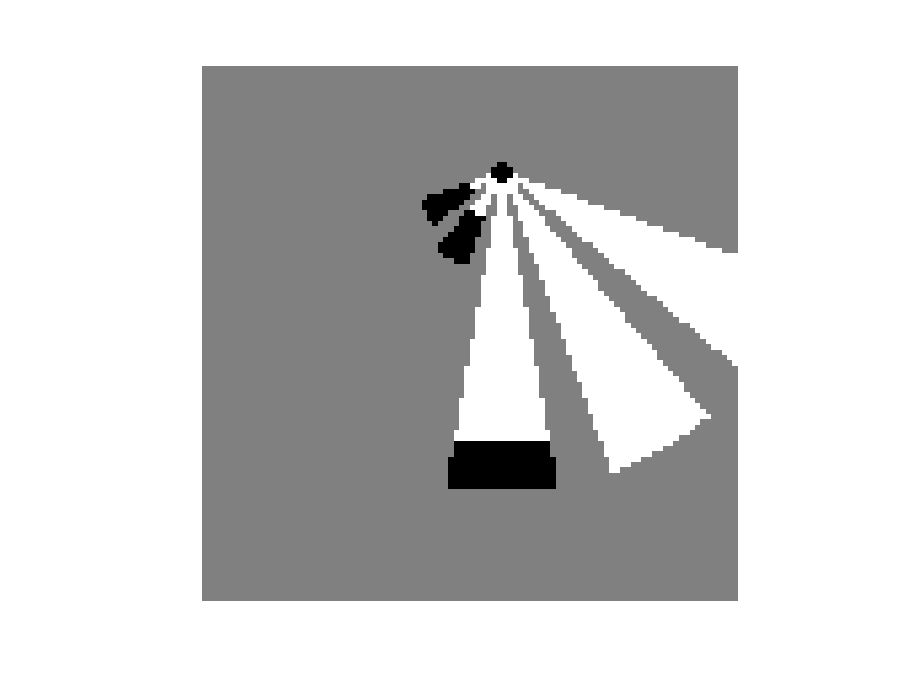
\includegraphics[width= 1.2\linewidth]{Figures/radar_data.eps}
    \caption{}
    \label{fig:SensorData}
\end{subfigure}
\begin{subfigure}[b]{0.48\linewidth}
    \centering
    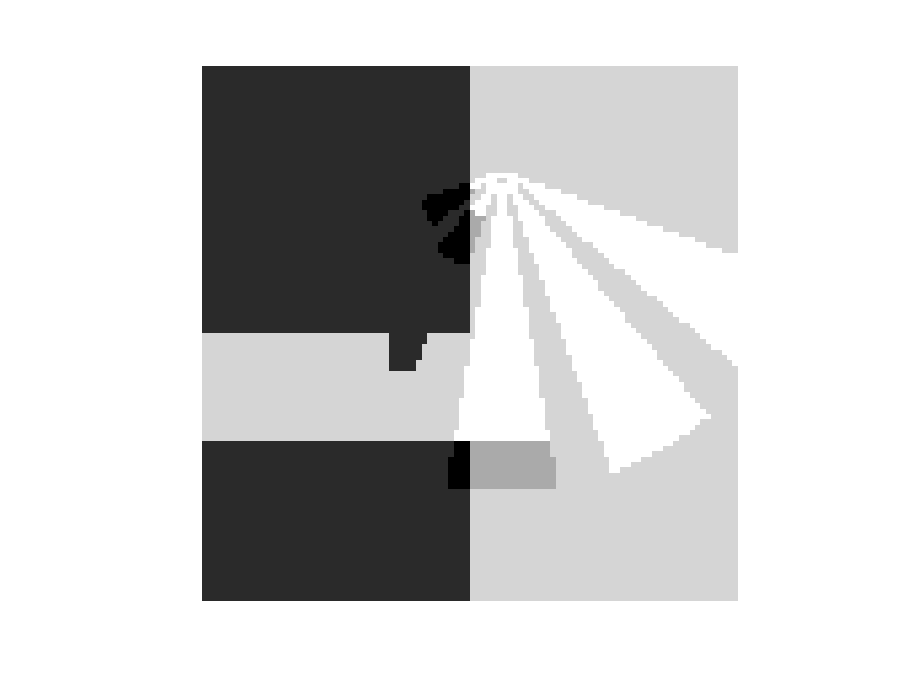
\includegraphics[width= 1.2\linewidth]{Figures/radar_data_superimposed.eps}
    \caption{}
    \label{fig:SuperimposedSensorData}
\end{subfigure}
\caption{Representation of the sensor-data from the stationary radar sensors. \ref{fig:SuperimposedSensorData} shows the sensordata superimposed on the true obstacle map }
\end{figure}


A grid-map is used to save the radar data over time. Each grid holds the probability of there being an object in that grid. The probabilities are simplified to only having three values,  1 if we have measured that there might be something in that grid, 0.5 if we have not measured the spot, and 0 if we know that the spot is safe. When a radar measurement is made, then all grids within the cone closer to the drone than the measured distance to the closest obstacle are marked as safe with a value 0. All cells further away than the measured distance that are within some penetration depth are assumed to contain an obstacle. These cells are marked as dangerous, 1, if they were previously marked as unknown. Since the radar may mark too many cells as potentially dangerous, the measurement of safe cells should trump a marked potentially dangerous cell. This way the drone will start with a restrictive map where too many cells are marked as dangerous, and after more measurements with different angles the safe cells will gradually be marked as safe.  Figure \ref{fig:Combined_obstacle_map} shows how the map can end up looking after the drone has flown along some route. 

\begin{figure}[!t]
\begin{subfigure}[b]{0.48\linewidth}
    \centering
    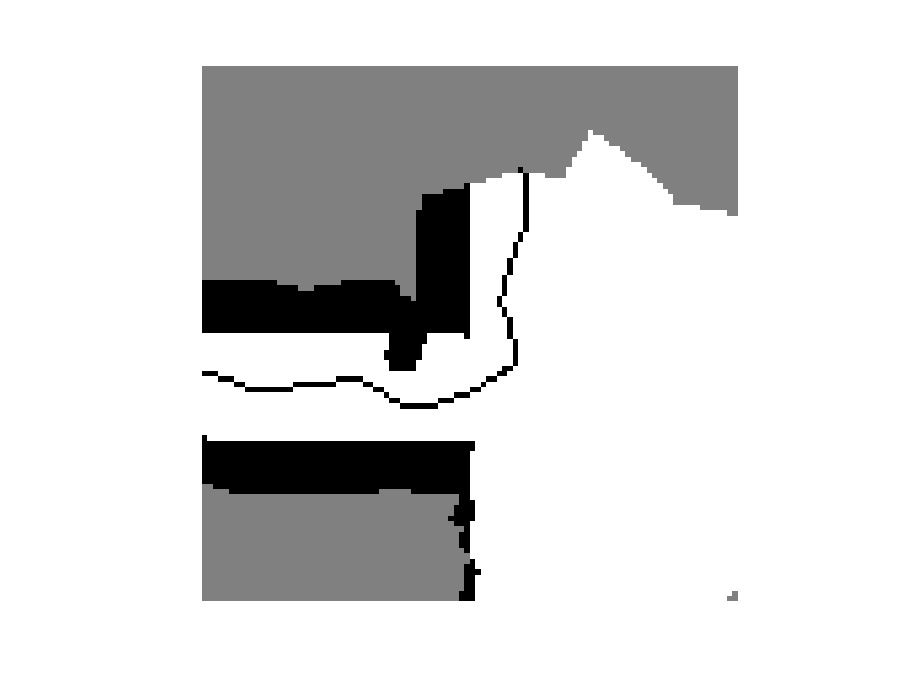
\includegraphics[width= 1.2\linewidth]{Figures/radar_after_flying}
    \caption{}
    \label{fig:Combined_obstacle_map}
\end{subfigure}
\begin{subfigure}[b]{0.48\linewidth}
    \centering
    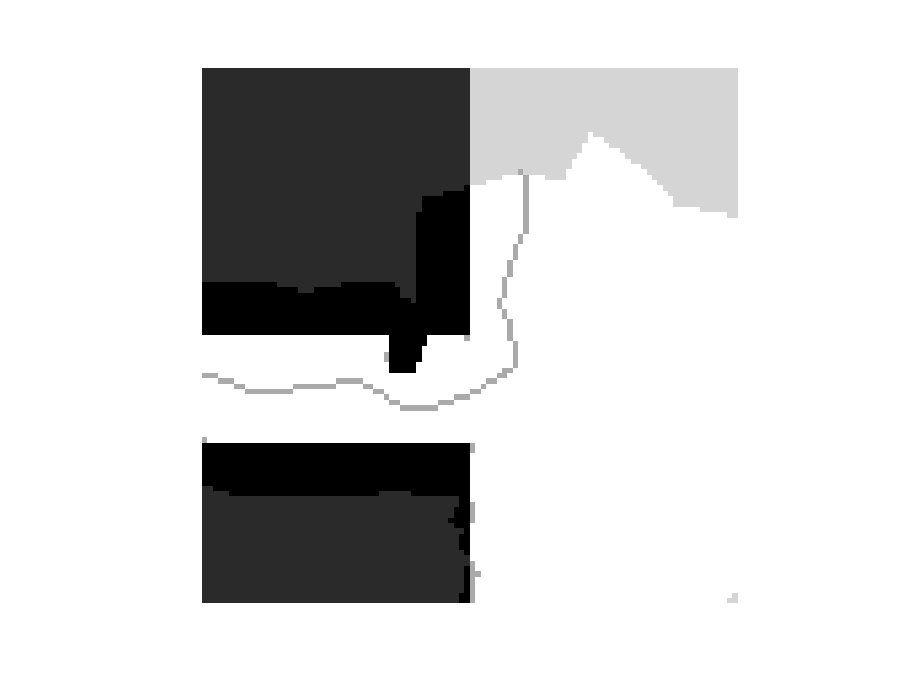
\includegraphics[width= 1.2\linewidth]{Figures/radar_after_flying_superimposed}
    \caption{}
\end{subfigure}
\caption{The obstacle map after flying along the marked path.  }
\end{figure}

The penetration depth should be designed large enough such that if the drone probability density function moves through it, then 95\% of Gaussian position curve should be inside the area marked as dangerous at some point. $\pm2 \sigma_p$, where $\sigma_p$ is the largest uncertainty in position over the time horizon, will encompass 95\% of the Gaussian curve that marks the uncertainty in position. In addition a margin has to be added due to the discrete time-steps to ensure that there exists a time-step when the curve is inside the marked area. The penetration depth should then be chosen as follows.
    \begin{equation}
        d_p = 4\sigma_p +dt v_0 \label{penetration_deapth}
    \end{equation}


This strategy for combining sensor data will not work in reality as it is not robust against measurement or position estimate errors. The cells should also give some sort of probability that there is an obstacle in the cell, and not the clean cut 0, 0.5, 1 probabilities it does now. The radar sensor model and combining of data requires further work. 